\documentclass[aspectratio=169]{beamer}

\usepackage[utf8]{inputenc}
\usecolortheme{beaver}
\usepackage{caption}
\usepackage{subcaption}
\usepackage{mathtools}
\usepackage{todonotes}
\usepackage{amsmath}
\usepackage{float}
\usepackage{bm}
\usepackage{listings}
\usepackage{ragged2e}
\usepackage{titlecaps}
\usepackage{fancyvrb}
\usepackage[export]{adjustbox}
\usepackage{minted}
\setminted{xleftmargin=1cm}
\def\ci{\perp\!\!\!\!\!\perp}

\newtheorem{proposition}{Proposition}
\Addlcwords{for a is but and with of in as the etc on to if}

\newcommand\github{
\includegraphics[height=2ex]{imgs/github.png}}
\newcommand\email{
\includegraphics[height=3ex]{imgs/email.png}}

\newcommand\blfootnote[1]{
    \begingroup
    \renewcommand\thefootnote{}\footnote{#1}
    \addtocounter{footnote}{-1}
    \endgroup
}

\setbeamertemplate{section in toc}{\inserttocsectionnumber.~\inserttocsection}
\usetheme{Boadilla}

\setbeamersize{text margin left=1em,text margin right=1em}
\makeatletter
\setbeamertemplate{footline}{%
    \leavevmode%
    \hbox{%
        \begin{beamercolorbox}[wd=.3\paperwidth,ht=2.25ex,dp=1ex,center]{author in head/foot}%
            \usebeamerfont{author in head/foot}\insertshortauthor\expandafter\beamer@ifempty\expandafter{\beamer@shortinstitute}{}{~~(\insertshortinstitute)}
        \end{beamercolorbox}%
        \begin{beamercolorbox}[wd=.55\paperwidth,ht=2.25ex,dp=1ex,center]{title in head/foot}%
            \usebeamerfont{title in head/foot}\insertshorttitle
        \end{beamercolorbox}%
        \begin{beamercolorbox}[wd=.15\paperwidth,ht=2.25ex,dp=1ex,right]{date in head/foot}%
            \usebeamerfont{date in head/foot}\insertshortdate{}\hspace*{2em}
            \insertframenumber{} / \inserttotalframenumber\hspace*{2ex} 
        \end{beamercolorbox}}%
        \vskip0pt%
    }
\makeatother

\title[Causal Inference using pgmpy]{Introduction to Casual Inference using pgmpy}
\author{Ankur Ankan}
\institute[]{Postdoctoral Researcher \\ Radboud University, The Netherlands}
\date{}

\begin{document}

\begin{frame}
	\maketitle
\end{frame}

\begin{frame}{Correlation Does not Imply Causation}
	\begin{figure}
		\center
		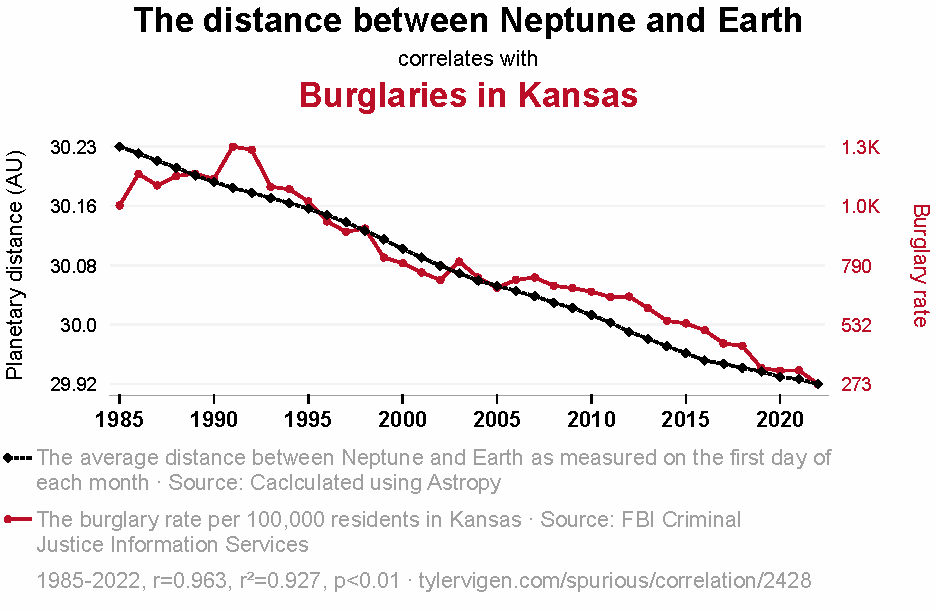
\includegraphics[scale=0.63]{imgs/spurious1.pdf}
	\end{figure}
	\blfootnote{https://tylervigen.com/spurious-correlations}
\end{frame}

\begin{frame}{Predictive vs Causal Modelling}
	\textbf{Predictive Modelling:}
		\begin{itemize}
			\item Interested in predicting outcome variables.
			\item Methods exploit correlation among variables.
		\end{itemize}
	\vspace{2em}
	\textbf{Causal Modelling:}
		\begin{itemize}
			\item Interested in identifying potential interventions and their effects (answering what-if questions).
			\item Methods learn the causal-effect relationships between variables.
			\item Just correlation information is not enough.
		\end{itemize}
\end{frame}


% \begin{frame}{Spurious Correlations}
% 	\begin{figure}
% 		\center
% 		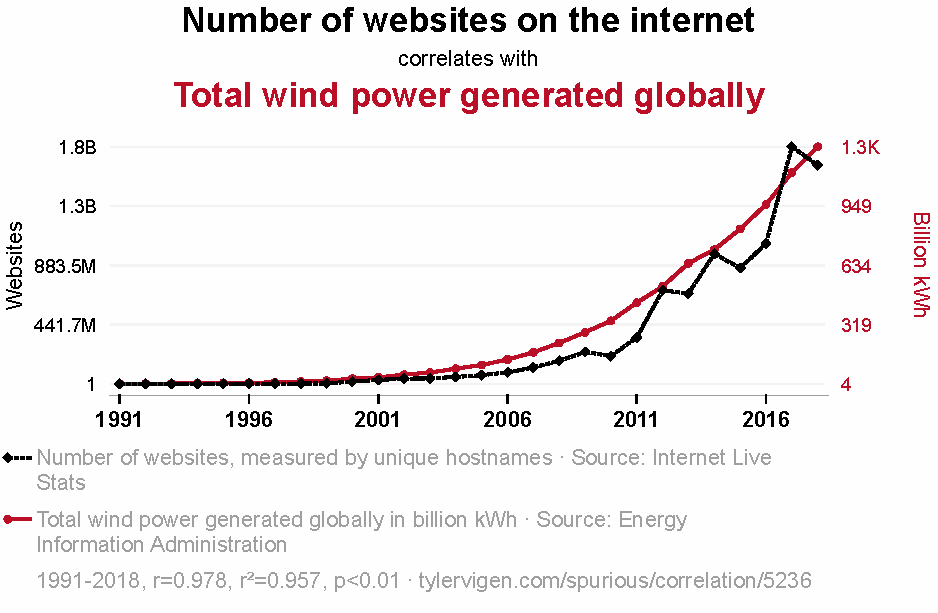
\includegraphics[scale=0.6]{imgs/spurious2.pdf}
% 	\end{figure}
% 	\blfootnote{https://tylervigen.com/spurious-correlations}
% \end{frame}

% \begin{frame}{Data Generating Process}
% 	\center{Causal Modelling requires understanding the data generating process}
% 	\vspace{1em}
% 	\begin{itemize}
% 		\item Confounder:  \begin{figure}[H] \includegraphics[scale=0.7, page=3]{figures.pdf}\end{figure}
% 		\item Mediator: \begin{figure}[H] \includegraphics[scale=0.7, page=8]{figures.pdf} \end{figure}
% 		\item Collider: \begin{figure}[H] \includegraphics[scale=0.7, page=9]{figures.pdf} \end{figure}
% 	\end{itemize}
% 	% \center{Would an intervention on Ice-cream Sales affect Drowning Cases?}
% \end{frame}

\begin{frame}{Example: Protein Signalling Causal Network \footnote{Sachs, Karen, et al. "Causal protein-signaling networks derived from multiparameter single-cell data." Science 308.5721 (2005): 523-529.}}
	\begin{columns}
		\begin{column}{0.5\textwidth}
			\begin{itemize}
				\item Models the concentration of signalling proteins in cells.
				\item Understanding the mechanism such as how the signals bring cellular responses.
				\item Insights on how signalling pathways are altered in diseases.
				\item Can be used to identify potential targets for therapeutic intervention.
			\end{itemize}
		\end{column}
		\begin{column}{0.5\textwidth}
			\begin{figure}
				\centering
				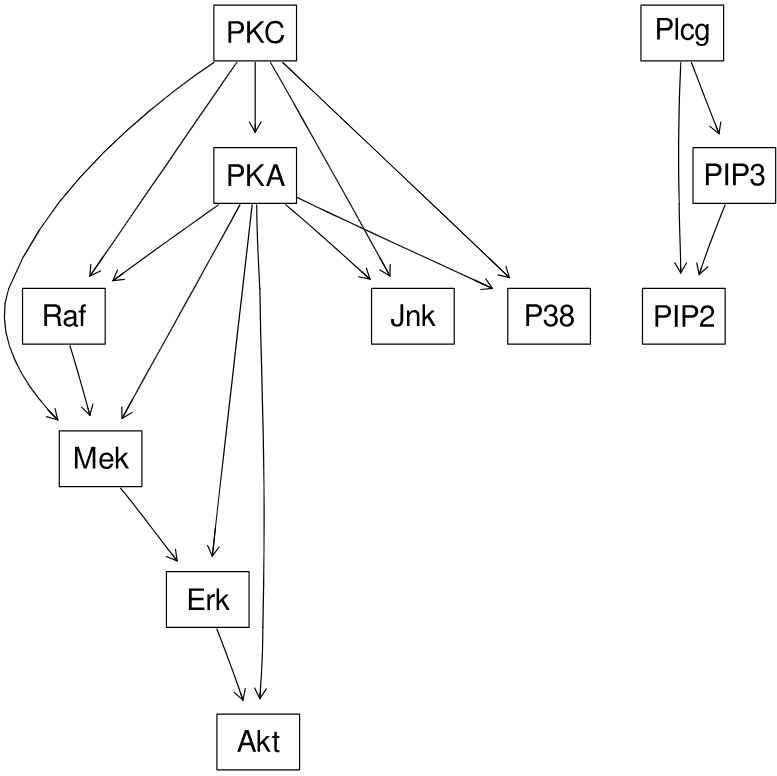
\includegraphics[scale=0.22]{imgs/sachs.png}
			\end{figure}
		\end{column}
	\end{columns}
\end{frame}

\begin{frame}{Examples}
	\begin{itemize}
		\item \textbf{Epidemiology:} Analyzing data on how different treatment or exposures affect health outcomes.
		\item \textbf{Economics and Social Sciences:} Understanding impacts of policy interventions and help in designing potential policies.
		\item \textbf{Machine Learning:} For interpretability, feature selection, making models robust to out of distribution predictions.
	\end{itemize}
\end{frame}

\begin{frame}{Two Main Frameworks}
	Mathematical frameworks for causal inference:
	\vspace{0.5em}
	\begin{itemize}
		\item \textbf{Potential Outcomes Framework} (a.k.a. Rubin's Casual Model)
			\begin{itemize}
				\item Usually interested in estimating causal effect.
				\item Provides robust statistical methods for estimation.
				\item Examples are Propensity Score based methods, Doubly robust estimators, meta learners, etc.
			\end{itemize}
	\end{itemize}
	\vspace{1em}
	\begin{itemize}
		\item \textbf{Directed Acyclic Graphs (DAGs)} / Structural Equation Models (SEMs)
			\begin{itemize}
				\item Causal graph (DAG) at the core.
				\item The causal graph can be used to define estimators for causal effects of interest.
				\item Causal graph can also be used for selecting appropriate variables in Potential Outcomes framework.
			\end{itemize}
	\end{itemize}
\end{frame}

\begin{frame}{Causal Inference Python Packages}
	\begin{columns}
		\begin{column}[T]{0.5 \textwidth}
			\center{\textbf{Potential Outcomes Frameworks}}
			\begin{itemize}
				\item Collection of estimation methods
					\begin{figure}
						
\includegraphics[scale=0.15]{imgs/dowhy.png}
					\end{figure}
				\item Doubly Robust Estimation
					\begin{figure}
						
\includegraphics[scale=0.1]{imgs/doubleml.png}
					\end{figure}
				\item Meta Learners: T/S/X-Learners
					\begin{figure}
						
\includegraphics[scale=0.3]{imgs/causalml.png}
					\end{figure}
			\end{itemize}

		\end{column}
		\vrule
		\begin{column}[T]{0.5 \textwidth}
			\center{\textbf{DAG Based Frameworks}}
			\begin{itemize}
				\item pgmpy
					\begin{figure}
						
\includegraphics[scale=0.15]{imgs/pgmpy.png}
					\end{figure}
				\item causal-learn
					\begin{figure}
						
\includegraphics[scale=0.2]{imgs/pywhy_logo.png}
					\end{figure}
				% \item casualnex
				% 	\begin{figure}
				% 		
\includegraphics[height=2cm, width=3cm, scale=0.15]{imgs/causalnex.png}
				% 	\end{figure}
			\end{itemize}
		\end{column}
	\end{columns}
\end{frame}


% \begin{frame}{pgmpy}
% 	\todo[inline]{Do I want to keep this slide}
% 	\begin{itemize}
% 		\item Support for mixed data.
% 		\item Practical methods to integrate expert knowledge.
% 		\item Extensible. Add your own scoring functions, conditional independence tests.
% 	\end{itemize}
% 
% 
% \begin{figure}[t]
% 	\centering
% 	\begin{tikzpicture}[inner sep=1pt]
% 	\tikzstyle{every node}=[align=left]
% 		\node (data)  at (0, 0) {Data};
% 		\node (dag)    at (5, 0) {DAG};
% 		\node (user)  at (5, 1.2) {Import / User Defined};
% 		\node (bn)    at (12, 0) {Parameterized BN};
% 		\node (test)  at (2.5, -0.8) {Model Testing};
% 		\node (iv)    at (3.7, -1.4) {Instrumental Variables};
% 		\node (as)    at (6, -0.8) {Adjustment Set};
% 		\node (sim)   at (9, -0.8) {Simulations};
% 		\node (ci)    at (9.8, -1.4) {Causal Inference};
% 		\node (pi)    at (11.2, -2) {Probabilistic Inference};
% 		\node (testp) at (14, -0.8) {Model Testing};
% 		\node (readwrite) at (12.8, -1.4) {Export};
% 		\node (read) at (12, 1.2) {Import / User Defined};
% 
% 		\draw[->] (data) edge [bend left=10] node [midway, above]{Structure Learning} (dag.west);
% 		\draw (dag.east) edge [->,bend left=10] node [midway, above]{Parameter Learning} (bn.west);
% 		\draw[->] (user.south) -- (dag.north);
% 		\draw[->] (dag.south) -- (test.north);
% 		\draw[->] (dag.south) -- (iv.north);
% 		\draw[->] (dag.south) -- (as.north);
% 		\draw[->] (bn.south) -- (pi.north);
% 		\draw[->] (bn.south) -- (ci.north);
% 		\draw[->] (bn.south) -- (sim.north);
% 		\draw[->] (bn.south) -- (testp.north);
% 		\draw[->] (bn.south) -- (readwrite.north);
% 		\draw[->] (read.south) -- (bn.north);
% 	\end{tikzpicture}
% 	\caption{Possible workflows in pgmpy for Bayesian Networks}
% 	\label{fig:pgmpy_workflow}
% \end{figure}
% \end{frame}

\begin{frame}{A General Workflow in the DAG Framework}
	\begin{figure}
		\centering
		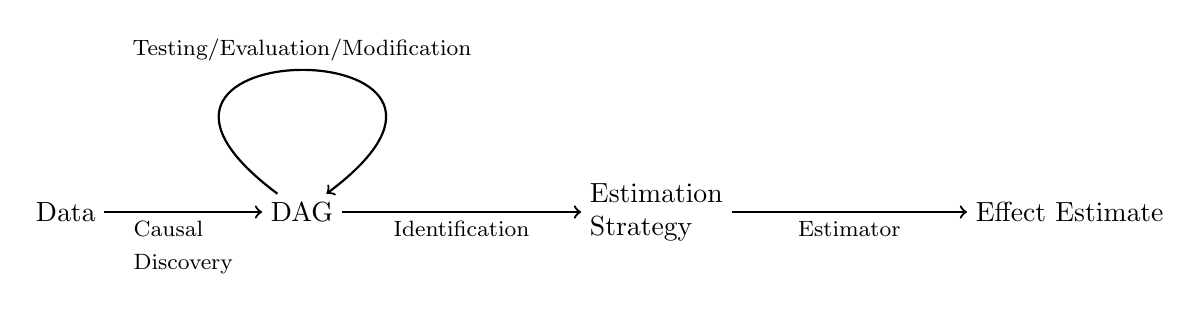
\begin{tikzpicture}[yscale=1, xscale=0.75, inner sep=3pt]
		\tikzstyle{every node}=[align=left]
			\node (data) at (0, 0) {Data};
			\node (dag) at (4, 0) {DAG};
			\node (estimand) at (10, 0) {Estimation \\ Strategy};
			\node (estimation) at (17, 0) {Effect Estimate};
	
			\draw[thick, ->] (data) to node[midway, below]{\footnotesize Causal \\ \footnotesize Discovery} (dag);
			\draw[thick, ->] (dag) to node[midway, below] {\footnotesize Identification} (estimand);
			\draw[thick, ->] (estimand) to node[midway, below] {\footnotesize Estimator} (estimation);
			\draw[thick, ->] (dag) [out=150, in=30, looseness=10] to node[midway, above] {\footnotesize Testing/Evaluation/Modification} (dag);
		\end{tikzpicture}
		\label{fig:workflow}
	\end{figure}
\end{frame}

% \begin{frame}{What does pgmpy provide}
% 	Will show how to perform each of these steps in pgmpy.
% 	\begin{itemize}
% 		\item Provides standardized implementations of commonly used algorithms.
% 		\item Practical methods methods.
% 		\item Extensible.
% 	\end{itemize}
% \end{frame}

\begin{frame}{Causal Discovery}
	\begin{figure}
		\centering
		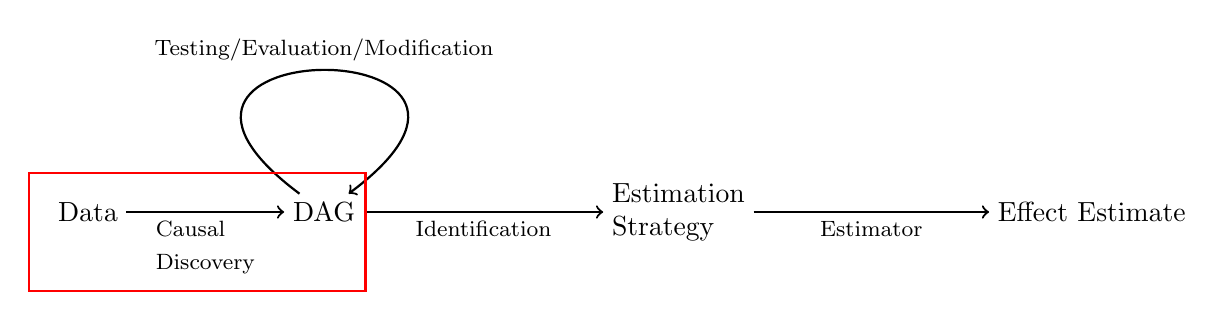
\begin{tikzpicture}[yscale=1, xscale=0.75, inner sep=3pt]
		\tikzstyle{every node}=[align=left]
			\node (data) at (0, 0) {Data};
			\node (dag) at (4, 0) {DAG};
			\node (estimand) at (10, 0) {Estimation \\ Strategy};
			\node (estimation) at (17, 0) {Effect Estimate};
	
			\draw[thick, ->] (data) to node[midway, below]{\footnotesize Causal \\ \footnotesize Discovery} (dag);
			\draw[thick, ->] (dag) to node[midway, below] {\footnotesize Identification} (estimand);
			\draw[thick, ->] (estimand) to node[midway, below] {\footnotesize Estimator} (estimation);
			\draw[thick, ->] (dag) [out=150, in=30, looseness=10] to node[midway, above] {\footnotesize Testing/Evaluation/Modification} (dag);

			\draw[draw=red, thick] (-1, -1) rectangle (4.7, 0.5);
		\end{tikzpicture}
		\label{fig:workflow1}
	\end{figure}
	\vspace{1em}
	\center \textbf{Casual Discovery: } Learn the causal graph (DAG) from the given data.
\end{frame}

\begin{frame}{Causal Discovery: Automated Algorithms}
	\begin{itemize}
		\item Many automated algorithms with nice asymptotic properties.
			\begin{itemize}
				\item \textbf{Constraint-based:} PC, Fast Causal Inference.
				\item \textbf{Score-based:} Greedy Equivalence Search, Hill-Climb Search.
				\item \textbf{Optimization-based:} NoTears, DAGMA.
			\end{itemize}
		\item However, difficult to use in practice.
			\begin{itemize}
				\item Unsupervised learning problem; no good way to check how good the learned graph is.
				\item Outputs are sensitive to algorithm, hyperparameters, and sample size.
				\item Many DAGs can represent the same observed correlation.
			\end{itemize}
	\end{itemize}
\end{frame}

\begin{frame}{Causal Discovery: Automated Algorithms}
	\textbf{Adult Income Dataset:}
	\vspace{2em}
	\begin{figure}
		\center
		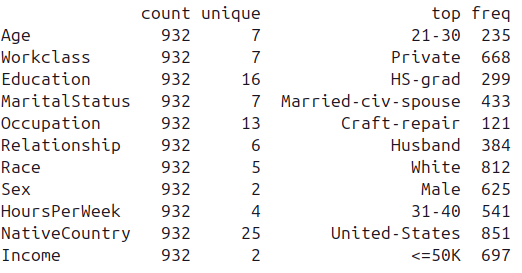
\includegraphics[scale=0.5]{imgs/adult_describe.png}
	\end{figure}
	\blfootnote{Becker,Barry and Kohavi,Ronny. (1996). Adult. UCI Machine Learning Repository.}
\end{frame}

\begin{frame}[fragile]{Causal Discovery: Automated Algorithms}
	\begin{columns}
		\begin{column}{0.45 \textwidth}
			\begin{minted}[linenos, fontsize=\footnotesize]{python}
from pgmpy.estimators import PC

est = PC(df)
dag = est.estimate(
	ci_test='chi_square'
)
			\end{minted}
			\vspace{3em}

			\begin{minted}[linenos, fontsize=\footnotesize]{python}
from pgmpy.estimators import HillClimbSearch

est = HillClimbSearch(df)
dag = est.estimate(
	scoring_method='bicscore'
)
			\end{minted}
		\end{column}
		\begin{column}{0.55 \textwidth}
			\begin{figure}
				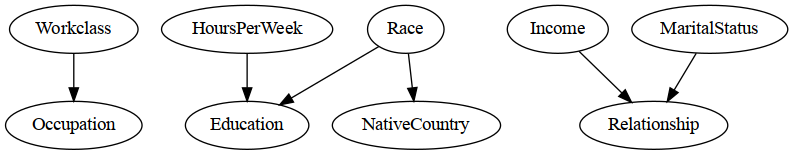
\includegraphics[scale=0.3]{imgs/adult_x2.png}
			\end{figure}
			\vspace{1em}
			\begin{figure}
				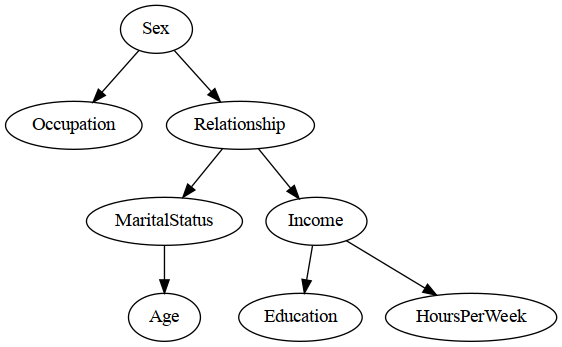
\includegraphics[scale=0.3]{imgs/adult_bic.png}
			\end{figure}
		\end{column}
	\end{columns}
\end{frame}

\begin{frame}[fragile]{Causal Discovery: Automated Algorithms}
	\begin{columns}
		\begin{column}{0.45 \textwidth}
			\begin{minted}[linenos, fontsize=\footnotesize]{python}
from pgmpy.estimators import PC

est = PC(df)
dag = est.estimate(
	ci_test='chi_square'
)
			\end{minted}
			\vspace{4em}

			\begin{minted}[linenos, fontsize=\footnotesize]{python}
from pgmpy.estimators import PC

est = PC(df)
dag = est.estimate(
	ci_test='pillai'
)
			\end{minted}
		\end{column}
		\begin{column}{0.55 \textwidth}
			\begin{figure}
				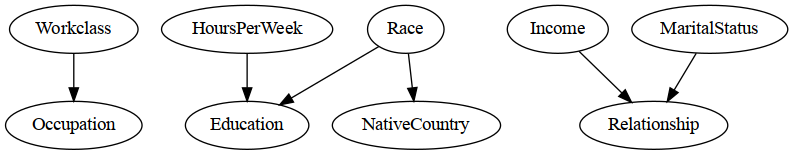
\includegraphics[scale=0.3]{imgs/adult_x2.png}
			\end{figure}
			\vspace{2em}
			\begin{figure}
				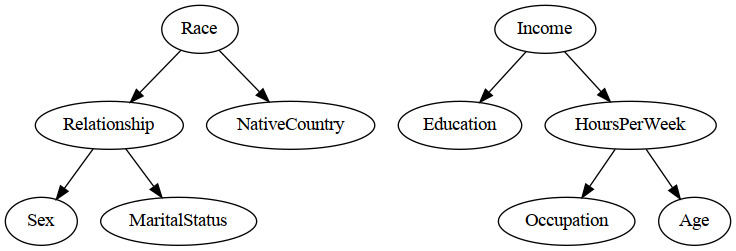
\includegraphics[scale=0.3]{imgs/adult_pillai.png}
			\end{figure}
		\end{column}
	\end{columns}


	% \begin{figure}
	% 	\begin{subfigure}{0.45\textwidth}
	% 		\centering
	% 		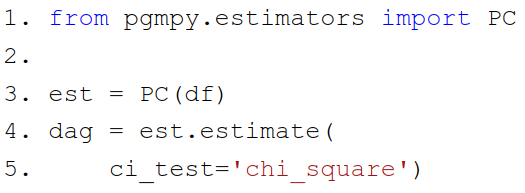
\includegraphics[scale=0.28]{imgs/pc_chisquare.png}
	% 	\end{subfigure}%
	% 	\begin{subfigure}{0.55 \textwidth}
	% 		\centering
	% 		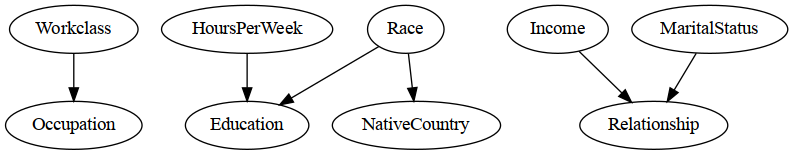
\includegraphics[scale=0.25]{imgs/adult_x2.png}
	% 	\end{subfigure}\vfill
	% 	\begin{subfigure}{0.45 \textwidth}
	% 		\centering
	% 		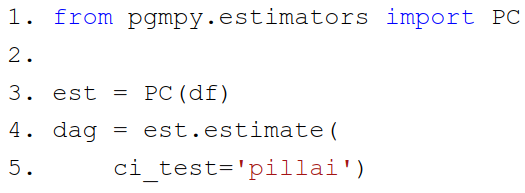
\includegraphics[scale=0.28]{imgs/pc_pillai.png}
	% 	\end{subfigure}%
	% 	\begin{subfigure}{0.55 \textwidth}
	% 		\centering
	% 		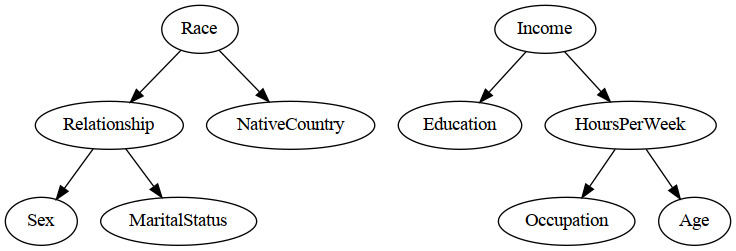
\includegraphics[scale=0.25]{imgs/adult_pillai.png}
	% 	\end{subfigure}
	% \end{figure}
\end{frame}

\begin{frame}{Causal Discovery: Problems Automated Algorithms}
	\begin{itemize}
		\item Difficult to choose the best algorithm/model.
		\item All algorithms usually make mistakes in finite sample scenario.
		\item Integrating expert knowledge can help.
	\end{itemize}

	\vspace{2em}

	Few ways to specify expert knowledge in pgmpy:
	\begin{enumerate}
		\item Blacklist edges
		\item Whitelist edges and fixed edges
		\item Specifying initial graph
		\item Temporal information (Upcoming)
	\end{enumerate}
	
\end{frame}

\begin{frame}[fragile]{Causal Discovery: Expert Knowledge Integration}
	\begin{figure}
		\begin{subfigure}{0.6 \textwidth}
			\begin{minted}[linenos, fontsize=\footnotesize]{python}
est = HillClimbSearch(df)
blist = [('Sex', 'MaritalStatus'),
	 ('MaritalStatus', 'Income'),
	 ('Income', 'Education'),
	 ('MaritalStatus', 'Age'),
	 ('Income', 'HoursPerWeek')]
dag = est.estimate(scoring_method='bicscore',
		   black_list=blist)
			\end{minted}
		\end{subfigure}%
		\begin{subfigure}{0.4 \textwidth}
			\centering
			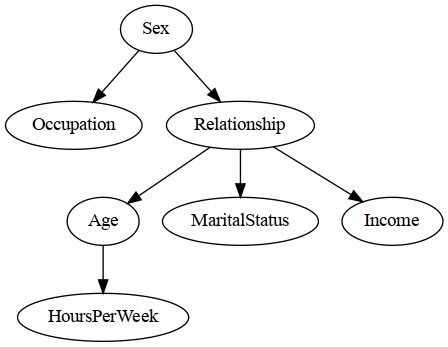
\includegraphics[scale=0.3]{imgs/adult_bic_blacklist.png}
		\end{subfigure}
	\end{figure}
\end{frame}

\begin{frame}[fragile]{Causal Discovery: Expert Knowledge Integration}
	\begin{figure}
		\begin{subfigure}{0.5 \textwidth}
			\begin{minted}[linenos, fontsize=\footnotesize]{python}
est = HillClimbSearch(df)
dag_bic_fixed = est.estimate(
    scoring_method='bicscore',
    fixed_edges=[
        ('HoursPerWeek', 'Income'),
	('Education', 'Income'),
	('Occupation', 'Income'),
	('Workclass', 'Income'),
	('Sex', 'Income'),
	]
)
			\end{minted}
		\end{subfigure}%
		\begin{subfigure}{0.5 \textwidth}
			\centering
			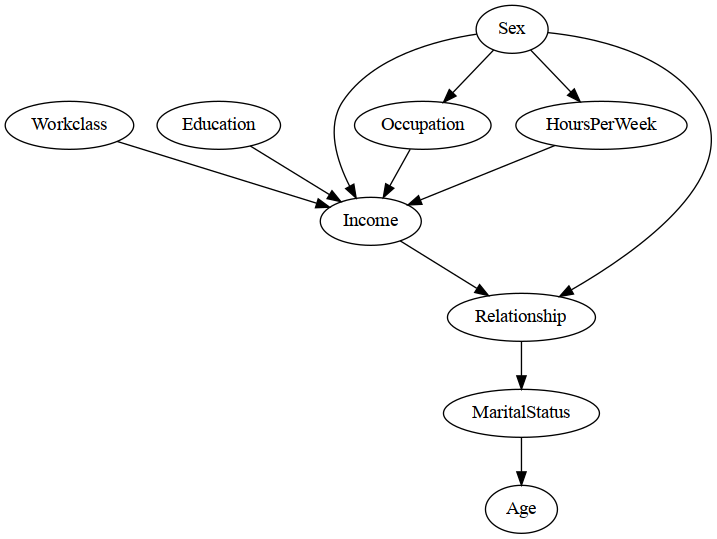
\includegraphics[scale=0.3]{imgs/adult_bic_fixed.png}
		\end{subfigure}
	\end{figure}
\end{frame}

\begin{frame}[fragile]{Causal Discovery: Expert Knowledge Integration}
	\begin{figure}
		\begin{subfigure}{0.5 \textwidth}
			\begin{minted}[linenos, fontsize=\footnotesize]{python}
from pgmpy.base import DAG
start_dag = DAG([
    ('Age', 'Income'),
    ('Age', 'Education'),
    ('Age', 'MaritalStatus'),
    ('Age', 'HoursPerWeek'),
    ('NativeCountry', 'Race'),
    ('HoursPerWeek', 'Income'),
    ('Education', 'Occupation'),
    ('Education', 'Income'),
    ('Education', 'Workclass'),
    ('Occupation', 'Income'),
    ('Sex', 'Income'),
    ('Relationship', 'MaritalStatus')
    ])
dag_bic_start = est.estimate(
    scoring_method='bicscore',
    start_dag=start_dag
)
			\end{minted}
		\end{subfigure}%
		\begin{subfigure}{0.5 \textwidth}
			\centering
			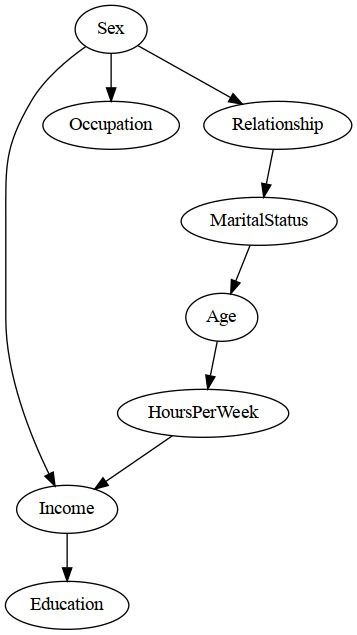
\includegraphics[scale=0.3]{imgs/adult_bic_start.png}
		\end{subfigure}
	\end{figure}
\end{frame}

\begin{frame}{Causal Discovery: Expert-In-The-Loop}
	\center{Since, causal discovery in practice is an iterative manual process, we designed an algorithm that works with interactive input from the user.}

	\vspace{2em}

	\begin{itemize}
		\item Combines score and constraint based algorithms.
		\item Iteratively asks user for expert knowledge.
		\item Reduces the amount of manual information that need to be provided.
		\item In absence of an expert, LLMs can be used.
	\end{itemize}
\end{frame}

\begin{frame}[fragile]{Causal Discovery: Expert-In-The-Loop}
	\begin{minted}[linenos, fontsize=\footnotesize]{python}
from pgmpy.estimators import ExpertInLoop

est_expert = ExpertInLoop(df)
dag_expert = est_expert.estimate(use_llm=False)
	\end{minted}
	\begin{figure}
		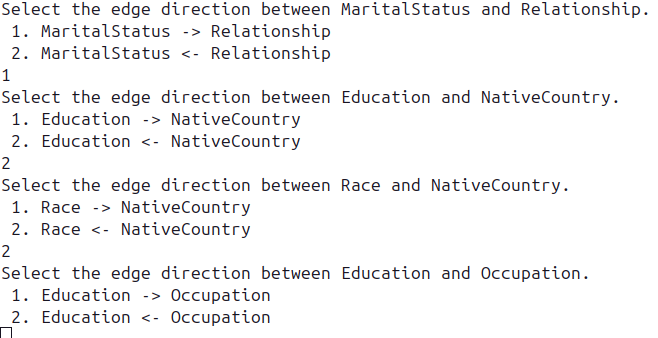
\includegraphics[scale=0.4, left]{imgs/expert_prompt.png}
	\end{figure}
\end{frame}

\begin{frame}[fragile]{Causal Discovery: Expert-In-The-Loop}
	\begin{minted}[fontsize=\scriptsize]{python}
descriptions = {
    "Age": "The age of a person",
    "Workclass": "The workplace where the person is employed such as ",
    		 "Private industry, or self employed",
    "Education": "The highest level of education the person has finished",
    "MaritalStatus": "The marital status of the person",
    "Occupation": "The kind of job the person does. For example, sales, craft repair, ",
    		  "clerical",
    "Relationship": "The relationship status of the person",
    "Race": "The ethnicity of the person",
    "Sex": "The sex or gender of the person",
    "HoursPerWeek": "The number of hours per week the person works",
    "NativeCountry": "The native country of the person",
    "Income": "The income i.e. amount of money the person makes",
}

dag_expert = est_expert.estimate(
    variable_descriptions=descriptions,
    use_llm=True)
	\end{minted}
\end{frame}

\begin{frame}{Causal Discovery: Expert-In-The-Loop}
	\begin{figure}
		\centering
		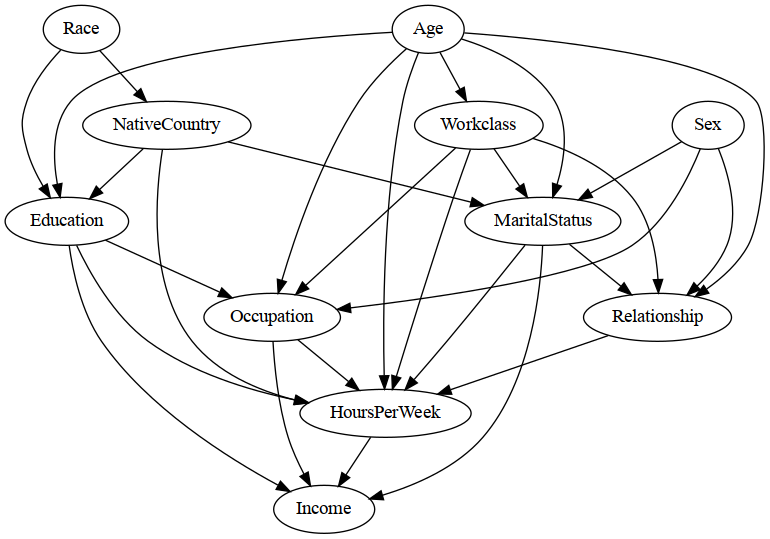
\includegraphics[scale=0.35]{imgs/adult_llm.png}
	\end{figure}
\end{frame}

% \begin{frame}{Bootstrapping}
% \end{frame}

\begin{frame}{Model Evaluation}
	\begin{figure}
		\centering
		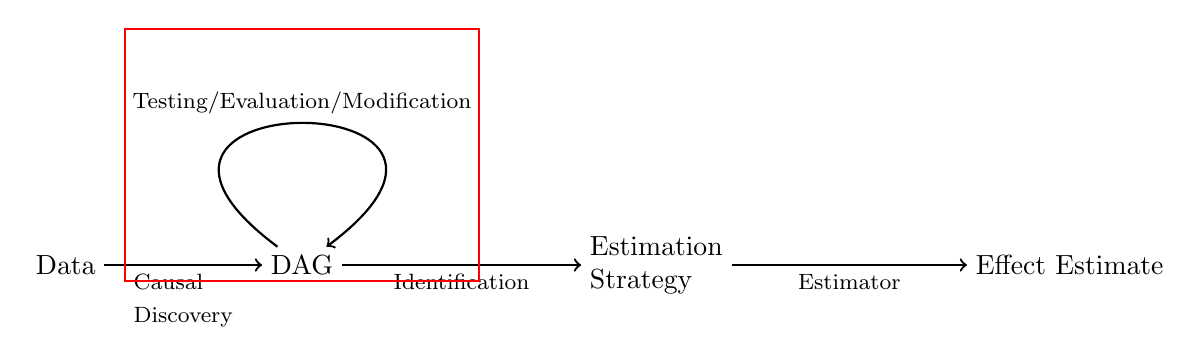
\begin{tikzpicture}[yscale=1, xscale=0.75, inner sep=3pt]
		\tikzstyle{every node}=[align=left]
			\node (data) at (0, 0) {Data};
			\node (dag) at (4, 0) {DAG};
			\node (estimand) at (10, 0) {Estimation \\ Strategy};
			\node (estimation) at (17, 0) {Effect Estimate};
	
			\draw[thick, ->] (data) to node[midway, below]{\footnotesize Causal \\ \footnotesize Discovery} (dag);
			\draw[thick, ->] (dag) to node[midway, below] {\footnotesize Identification} (estimand);
			\draw[thick, ->] (estimand) to node[midway, below] {\footnotesize Estimator} (estimation);
			\draw[thick, ->] (dag) [out=150, in=30, looseness=10] to node[midway, above] {\footnotesize Testing/Evaluation/Modification} (dag);

			\draw[draw=red, thick] (1, -0.2) rectangle (7, 3);
		\end{tikzpicture}
		\label{fig:workflow2}
	\end{figure}

	\begin{itemize}
		\item As causal discovery algorithms make mistakes, important to test and modify learned models.
	\end{itemize}
\end{frame}

\begin{frame}{Model Evaluation}
	\begin{itemize}
		\item Causal Discovery is similar to unsupervised learning problem.
		\item Do not have access to ground truth data.
		\item Ad-hoc methods to determine how well the model fits the data.
	\end{itemize}

	\vspace{2em}

	\center{pgmpy implements a few methods to test and compare models.}
\end{frame}

\begin{frame}{Model Evaluation: Implied Conditional Independences (CIs)}
	\begin{figure}
		\centering
		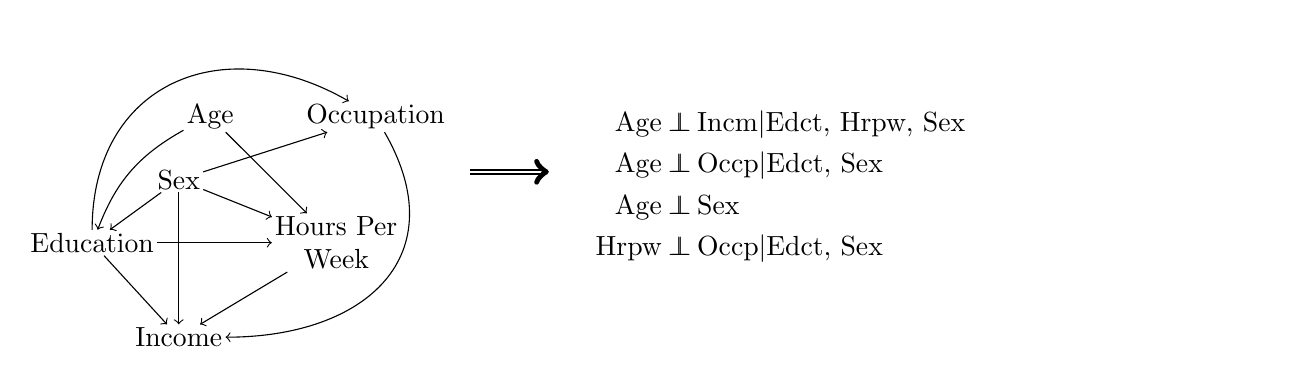
\begin{tikzpicture}
			\begin{scope}[xshift=1cm, yshift=0.7cm, scale=1]
			\tikzstyle{every node}=[align=center, inner sep=1pt]
				\node (sex) at (-0.7, -0.8) {Sex};
				\node (age) at (-0.3, 0) {Age};
				\node (ed) at (-1.8, -1.6) {Education};
				\node (occ) at (1.8, 0) {Occupation};
				\node (hrpw) at (1.3, -1.6) {Hours Per \\ Week};
				\node (income) at (-0.7, -2.8) {Income};
			
				\draw[->]  (age) to[bend right=20] (ed);
				\draw[->]  (sex) to (ed);
				\draw[->]  (age) to (hrpw);
				\draw[->]  (ed) to (hrpw);
				\draw[->]  (sex) to (hrpw);
				\draw[->]  (ed) to (income);
				\draw[->]  (hrpw) to (income);
				\draw[->]  (occ) to[out=300, in=0, looseness=1.4] (income.east);
				\draw[->]  (sex) to (income);
				\draw[->]  (ed) to[out=90, in=150, looseness=1.3] (occ);
				\draw[->]  (sex) to (occ);	
			\end{scope}
			\draw[thick, ->, double] (4,0) -- (5,0);
			\node[rectangle, align=center, inner sep=1pt] at (8, 0) {
				\begin{minipage}{\textwidth}
					\begin{equation*}
						\begin{split}
							\textnormal{Age} &\ci \textnormal{Incm} \rvert \textnormal{Edct, Hrpw, Sex} \\
							\textnormal{Age} &\ci \textnormal{Occp} \rvert \textnormal{Edct, Sex} \\
							\textnormal{Age} &\ci \textnormal{Sex} \\
							\textnormal{Hrpw} &\ci \textnormal{Occp} \rvert \textnormal{Edct, Sex} \\
						\end{split}
					\end{equation*}
				\end{minipage}
				};
		\end{tikzpicture}
	\end{figure}

	\vspace{1em}
	\begin{itemize}
		\item Each missing edge implies a Conditional Independence (CI).
		\item Statistical tests can be used to test whether the independence statement holds in the data.
		\item Models can be modified based on these tests.
	\end{itemize}

\end{frame}

\begin{frame}{Model Evaluation: Implied Conditional Independences (CIs)}
	\begin{figure}
		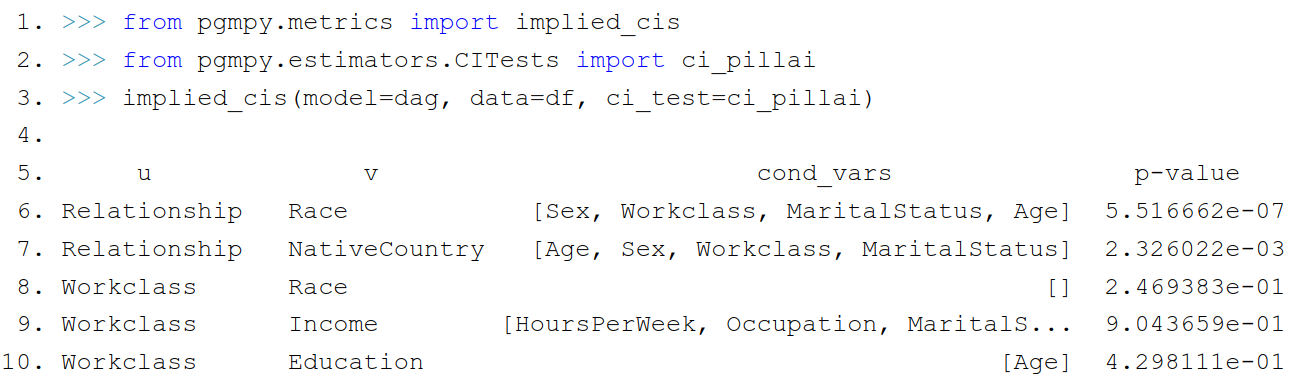
\includegraphics[scale=0.27]{imgs/implied_cis.png}
	\end{figure}
\end{frame}

\begin{frame}{Model Evaluation: Fisher's C Test}
	\begin{itemize}
		\item Combines the implied CI tests to summarize it into a single p-value.
		\item Using some significance threshold, we can decide whether the model fits well to the data.
	\end{itemize}
	\vspace{2em}
	\begin{figure}
		\centering
		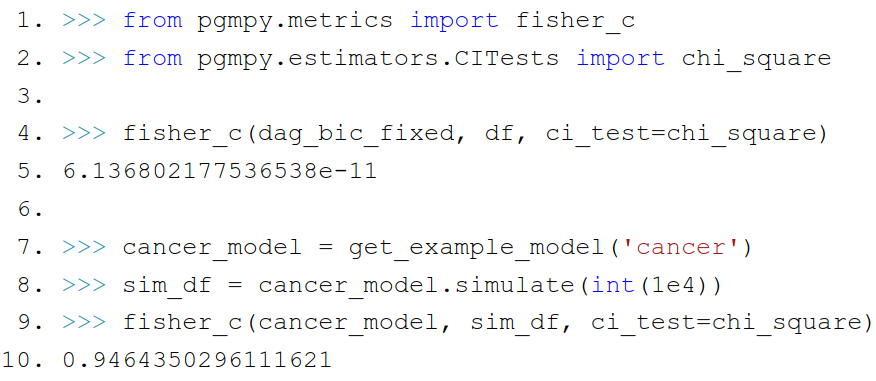
\includegraphics[scale=0.3]{imgs/fisherc.png}
	\end{figure}
\end{frame}

\begin{frame}{Model Evaluation: Correlation Score}
	\begin{itemize}
		\item How much of the observed correlation in the data is explained by the model.
		\item Compares whether variables that are correlated in data
			are also correlated in the model.
		\item Computes the F1-score based on this comparison.
	\end{itemize}
	\vspace{2em}
	\begin{figure}
		\centering
		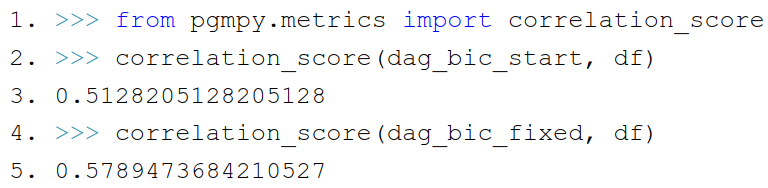
\includegraphics[scale=0.3]{imgs/corr_score.png}
	\end{figure}

\end{frame}


\begin{frame}{Model Evaluation: Structure Score Metrics}
	\begin{itemize}
		\item Scores the network structure based on how well they fit to data.
		\item Useful for comparing multiple models.
	\end{itemize}
	\vspace{1em}
	\begin{figure}
		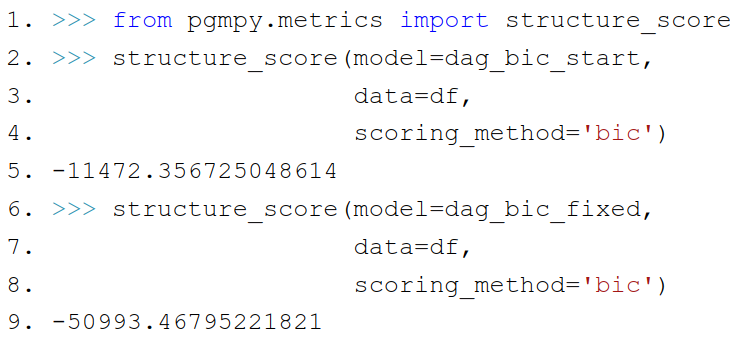
\includegraphics[scale=0.3]{imgs/structure_score.png}
	\end{figure}
\end{frame}

% \begin{frame}{Causal Discovery Algorithms learn a CPDAG}
% 	\begin{figure}
% 	\end{figure}
% 	
% 	\begin{itemize}
% 		\item Trying to learn a network structure which matches the covariance
% 			structure.
% 		\item Multiple networks can represent the same casual structure.
% 		\item Structure learning algorithms usually a DAG.
% 	\end{itemize}
% 
% 	Pairwise edge orientation rules.
% \end{frame}
% 
% \begin{frame}{Minimal Orientation}
% \end{frame}


% \begin{frame}{Using learned DAG in the PO framework}
% 	As DAGs explicitly show all the information, it can be used to make
% 	decisions in the PO framework as well.
% 
% 	The graph can be put into pywhy as well.
% \end{frame}

\begin{frame}{Identification}
	\begin{figure}
		\centering
		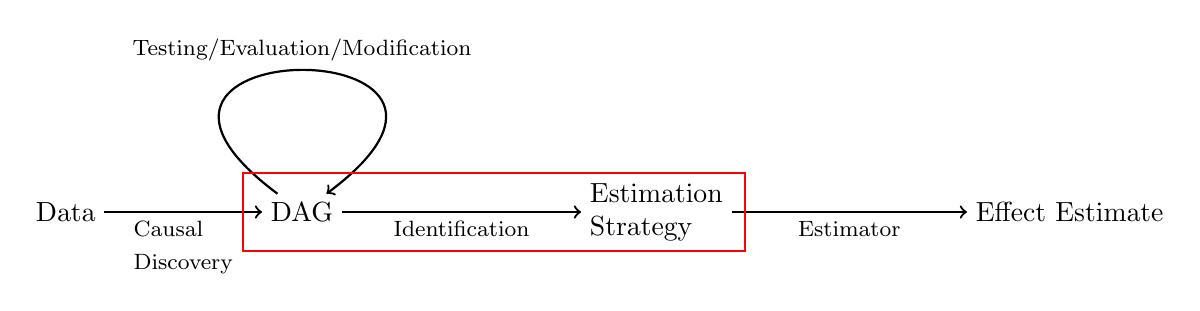
\begin{tikzpicture}[yscale=1, xscale=0.75, inner sep=3pt]
		\tikzstyle{every node}=[align=left]
			\node (data) at (0, 0) {Data};
			\node (dag) at (4, 0) {DAG};
			\node (estimand) at (10, 0) {Estimation \\ Strategy};
			\node (estimation) at (17, 0) {Effect Estimate};
	
			\draw[thick, ->] (data) to node[midway, below]{\footnotesize Causal \\ \footnotesize Discovery} (dag);
			\draw[thick, ->] (dag) to node[midway, below] {\footnotesize Identification} (estimand);
			\draw[thick, ->] (estimand) to node[midway, below] {\footnotesize Estimator} (estimation);
			\draw[thick, ->] (dag) [out=150, in=30, looseness=10] to node[midway, above] {\footnotesize Testing/Evaluation/Modification} (dag);

			\draw[draw=red, thick] (3, -0.5) rectangle (11.5, 0.5);
		\end{tikzpicture}
		\label{fig:workflow3}
	\end{figure}
	\begin{itemize}
		\item \textbf{Identification}: Is the causal effect of interest estimable?
		\item Everything is identified if all variables are observed.
	\end{itemize}
\end{frame}

\begin{frame}{Identification: do-calculus}
	\begin{figure}
		\begin{subfigure}{0.5 \textwidth}
			\centering
			\includegraphics[page=1]{figures.pdf}
		\end{subfigure}%
		\begin{subfigure}{0.5 \textwidth}
			\centering
			\includegraphics[page=2]{figures.pdf}
		\end{subfigure}
		\label{fig:idnent}
		% \caption{\center{(Left) $ U $ is unobserved; $\beta$ is unidentifiable. (Right) $ U $ is observed; $ \beta $ is identifiable.}}
	\end{figure}

	\begin{itemize}
		\item Theoretically, do-calculus provides a complete solution to identification.
		\item do-calculus can give an estimand for every identified causal effect.
		\item However, no efficient algorithms to get these estimands using do-calculus.
		\item In practice, we rely on a set of simpler identification strategies that work in special cases.
	\end{itemize}
\end{frame}

\begin{frame}{Identification: Backdoor Criterion}
	\begin{itemize}
		\item For cases when biasing paths can be blocked by conditioning.
		\item Finds adjustment variables to block confounding paths.
	\end{itemize}
	\begin{figure}
		\begin{subfigure}[c]{0.5\textwidth}
			\centering
			\includegraphics[page=4]{figures.pdf}
		\end{subfigure}%
		\begin{subfigure}[c]{0.5 \textwidth}
			\begin{equation*}
				\beta_{xy}: Y \sim X + U
			\end{equation*}
		\end{subfigure}
	\end{figure}

	\begin{figure}
		\centering
		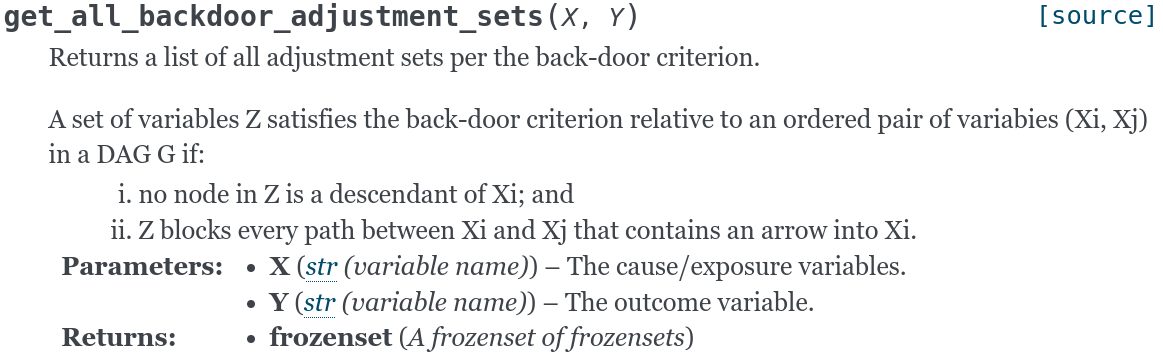
\includegraphics[scale=0.25]{imgs/backdoor.png}
	\end{figure}

\end{frame}

\begin{frame}{Identification: Front-door Criterion}
	\begin{itemize}
		\item Used for scenarios when there are mediator variables.
		\item Double application of backdoor criterion.
	\end{itemize}
	\begin{figure}
		\begin{subfigure}[c]{0.5 \textwidth}
			\centering
			\includegraphics[page=5]{figures.pdf}
		\end{subfigure}%
		\begin{subfigure}[c]{0.5 \textwidth}
			\centering
			\begin{equation*}
				\begin{split}
					\beta_{xm}:& M \sim X \\
					\beta_{my}:& Y \sim M + X \\
					\beta_{xy} =& \beta_{xm}\beta_{my}
				\end{split}
			\end{equation*}
		\end{subfigure}
	\end{figure}

	\begin{figure}
		\centering
		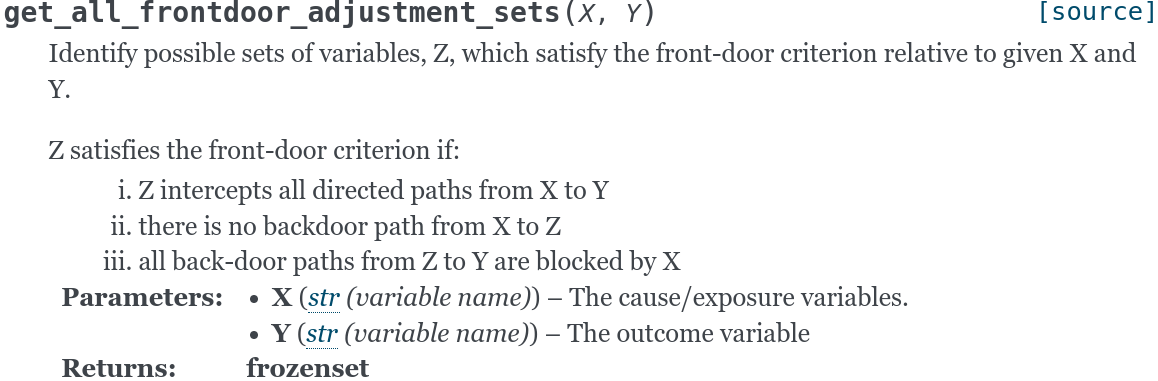
\includegraphics[scale=0.25]{imgs/frontdoor.png}
	\end{figure}
\end{frame}

\begin{frame}{Identification: Instrumental Variables}
	\begin{itemize}
		\item When there are variables in the model that are correlated
			with the outcome variable only through the exposure
			variable.
	\end{itemize}
	\begin{figure}
		\begin{subfigure}[c]{0.5 \textwidth}
			\centering
			\includegraphics[page=6]{figures.pdf}
		\end{subfigure}%
		\begin{subfigure}[c]{0.5 \textwidth}
			\begin{equation*}
				\begin{split}
					\beta_{zx} \beta_{xy}:& Y \sim Z \\
					\beta_{zx}:& X \sim Z \\
					\beta_{xy} =& \frac{\beta_{zx}\beta_{xy}}{\beta_{zx}} \\
				\end{split}
			\end{equation*}
		\end{subfigure}
	\end{figure}

	\begin{figure}
		\centering
		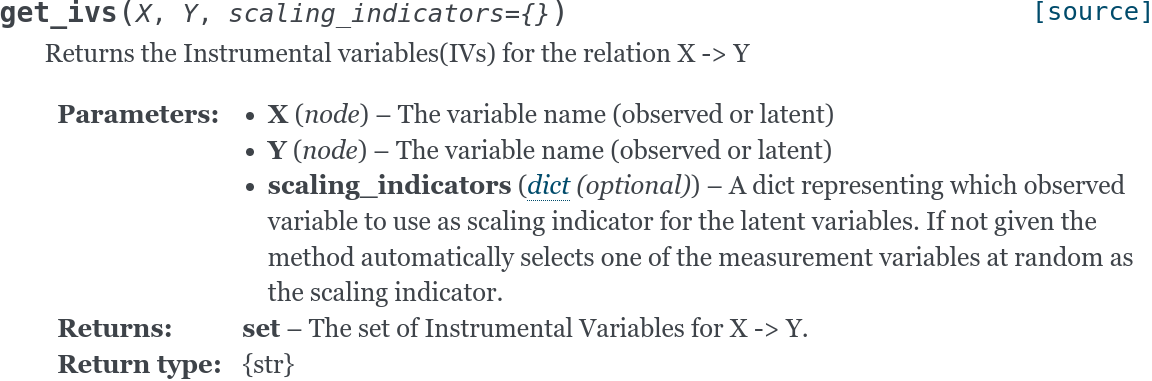
\includegraphics[scale=0.25]{imgs/ivs.png}
	\end{figure}
\end{frame}

\begin{frame}{Estimation}
	\begin{figure}
		\centering
		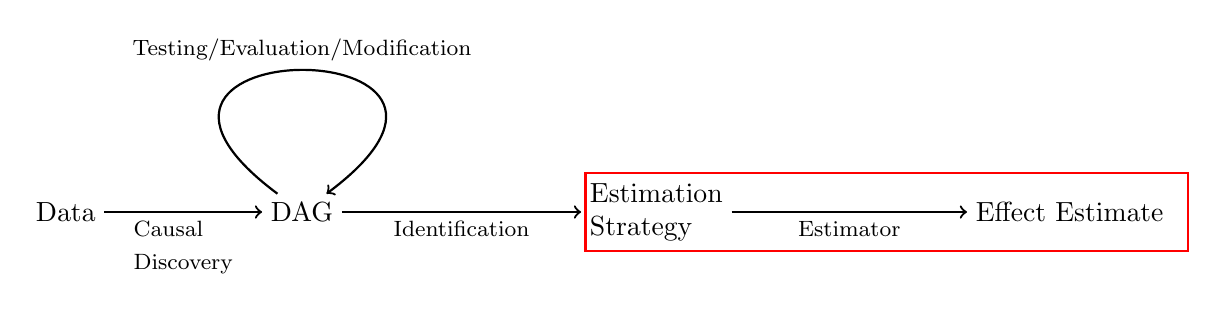
\begin{tikzpicture}[yscale=1, xscale=0.75, inner sep=3pt]
		\tikzstyle{every node}=[align=left]
			\node (data) at (0, 0) {Data};
			\node (dag) at (4, 0) {DAG};
			\node (estimand) at (10, 0) {Estimation \\ Strategy};
			\node (estimation) at (17, 0) {Effect Estimate};
	
			\draw[thick, ->] (data) to node[midway, below]{\footnotesize Causal \\ \footnotesize Discovery} (dag);
			\draw[thick, ->] (dag) to node[midway, below] {\footnotesize Identification} (estimand);
			\draw[thick, ->] (estimand) to node[midway, below] {\footnotesize Estimator} (estimation);
			\draw[thick, ->] (dag) [out=150, in=30, looseness=10] to node[midway, above] {\footnotesize Testing/Evaluation/Modification} (dag);

			\draw[draw=red, thick] (8.8, -0.5) rectangle (19, 0.5);
		\end{tikzpicture}
		\label{fig:workflow4}
	\end{figure}

	\begin{itemize}
		\item Identification methods give the estimand.
		\item Any estimator can be used to make the estimates.
		\item Usually linear models are used for their interpretability.
	\end{itemize}
\end{frame}

\begin{frame}
	\Huge Some other features.
\end{frame}

\begin{frame}{Simulations}
	\begin{itemize}
		\item Parameterized DAGs are generative models.
		\item Simulated data can be used to evaluate methods.
		\item Can be used for approximate inference.
		\item Helpful in explaining concepts like confounding, bias, etc.
	\end{itemize}
	\begin{figure}
		\centering
		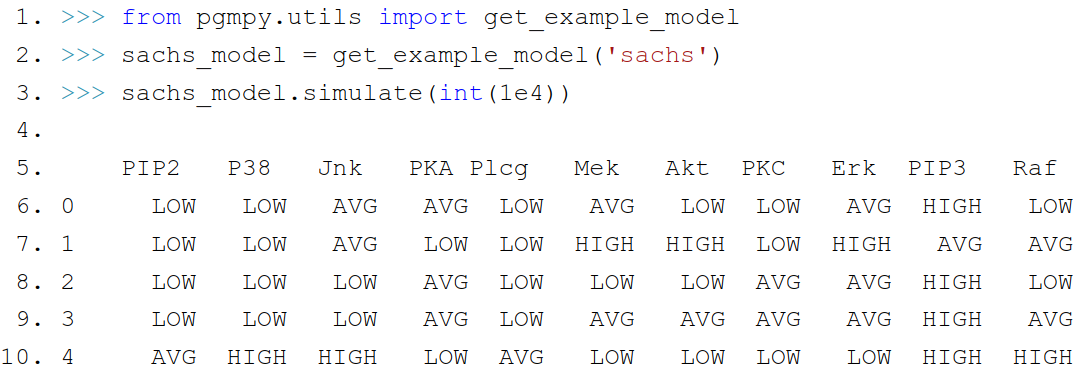
\includegraphics[scale=0.3]{imgs/data_sim.png}
	\end{figure}
\end{frame}
\begin{frame}{Simulations}
	\begin{figure}
		\centering
		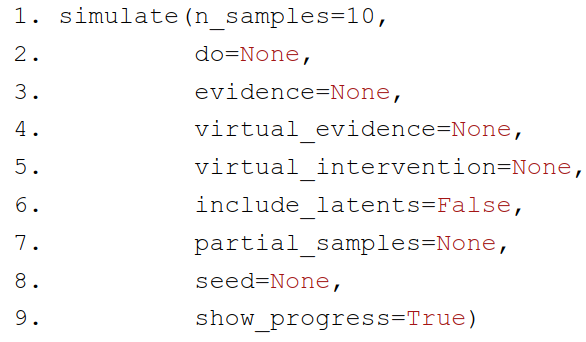
\includegraphics[scale=0.3]{imgs/simulate_fun.png}
	\end{figure}
\end{frame}

\begin{frame}{Extensibility}
	\begin{itemize}
		\item Causal Inference is a very active field of research.
		\item pgmpy offers easy ways to extend/modify algorithms.
		\item Methods accept custom functions as argument.
		\item Base classes make it easier to implement new algorithms and can be plugged into other functionality.
	\end{itemize}
	\vspace{1em}
	\begin{figure}
		\centering
		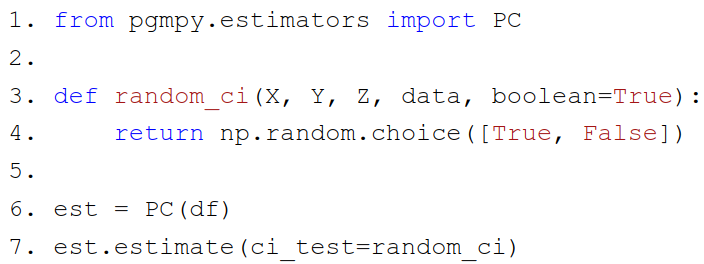
\includegraphics[scale=0.3]{imgs/extend.png}
	\end{figure}
\end{frame}

\begin{frame}{Future Plans}
	\begin{itemize}
		\item Implementing more practical methods such as bootstrapping, better conditional independence tests.
		\item Adding more commonly used causal discovery, and identification algorithms.
	\end{itemize}
\end{frame}

% \begin{frame}
% 	\begin{itemize}
% 		\item DAG based causal inference is great for interpretability, making 
% 			our data assumptions explicit.
% 		\item Constructing the model from data can be challenging.
% 		\item Often requires some addition of expert knowledge.
% 	\end{itemize}
% \end{frame}

\begin{frame}
	\center{\Huge {Thank you}}
	\vspace{5em}

	\github : pgmpy/pgmpy
	\vspace{1em}

	\email : ankurankan@gmail.com
\end{frame}

% \begin{frame}{Extra slide}
% 	When to use PO vs DAG framework?
% \end{frame}
% 
% \begin{frame}
% 	How does it compare to Shapley values 
% 	\begin{itemize}
% 		\item Still prediction based. Does not matter if perturbing direct effect variable or undirect.
% 		\item Can show an example where Shapley values would still find an association, but causal inference would not. The standard confounding case.
% 	\end{itemize}
% \end{frame}
\end{document}
